\chapter{Estudo de Caso}
O estudo de caso que será usado para validar os métodos de Aprendizagem de Máquina com Aprendizagem Incremental é baseado em um problema real do Ministério da Agricultura, Pecuária e Abastecimento (MAPA). Este ministério é responsável  "pela gestão das políticas públicas de estímulo à agropecuária, pelo fomento do agronegócio e pela regulação e normatização de serviços vinculados ao setor" \cite{mapa}. Um dos objetivos do MAPA é garantir a segurança alimentar do povo brasileiro além de suportar a produção de exportação, garantindo o sucesso dos produtos brasileiros no mercado internacional.

Uma das atribuições do Ministério da Agricultura é velar pela segurança dos produtos agropecuários que entram e saem do país. Para isto existe o Sistema de Vigilância Agropecuária Internacional (Vigiagro) que é vinculado a Secretaria de Defesa Agropecuária. O Vigiagro "atua na inspeção e fiscalização do trânsito internacional de vegetais, seus produtos e subprodutos. A fiscalização é feita nos portos, aeroportos internacionais, postos de fronteira e aduanas especiais" \cite{vigiagro}.

Neste contexto o vigiagro tem a atribuição fiscalizar todas as importações e exportações de produtos agropecuários do Brasil. Cada importação/exportação gera um requerimento, um documento onde o exportador/importador informa que realizará uma transação comercial internacional de um produto que está sobre vigilância do Vigiagro. Todos os requerimentos são inseridos no Sistema de Informações Gerenciais (SIGVIG). Os funcionários do Ministério então verificam vários itens, alguns de cunho documental e outros de cunho físico do produto comercializado. Caso haja alguma inconformidade o fiscal que avalia o requerimento gera um Termo de Ocorrência (TO) explicando a natureza e razão do erro encontrado, seja documental ou físico. Caso não haja nenhum erro o TO gerado consta que não houve erro em nenhum dos critérios avaliados.

O problema de todo este processo é que no Brasil a quantidade de requerimentos gerada é enorme. O processo de fiscalização é extremamente trabalhoso e demanda muito tempo dos fiscais. Propõe-se utilizar métodos de Aprendizado de Máquina para criar um sistema que auxilie na fiscalização, diminuindo o tempo de processamento dos requerimentos e aumentando a qualidade da fiscalização. Este sistema deve ser capaz de analisar todos os requerimentos feitos associados com o resultado da fiscalização, deferimento ou indeferimento do processo. Através desta análise deve ser possível classificar os exportadores/importadores em três categorias: Alta Conformidade, Média Conformidade e Baixa Conformidade. Através destes três rótulos é possível criar políticas de fiscalização que foquem os esforços nos comerciantes que geralmente possuem baixa conformidade em seus requerimentos, fazendo com que os comerciantes que sempre possuem conformidade tenham seus processos agilizados e os que possuem baixa conformidade tenham seus requerimentos avaliados cuidadosamente. 

Os dados que são relevantes para a construção deste sistema classificador é proveniente da união de dois relatórios gerados pelo SIGVIG: O relatório de todos Requerimentos de um determinado período de tempo com todos os Termos de Ocorrência correspondentes a estes requerimentos. A combinação destes dois relatórios fornece as características do importador/exportador, as características do produto negociado e o resultado da avaliação deste requerimento pelos fiscais do MAPA.

A figura 12 é um exemplo de como será o conjunto de dados que deve ser avaliado pelo sistema classificador. Ela consiste em 37 registros que são a combinação das informações entre Requerimentos e Termos de Ocorrência de produtos de importação.

\begin{figure}[!h]
\centering
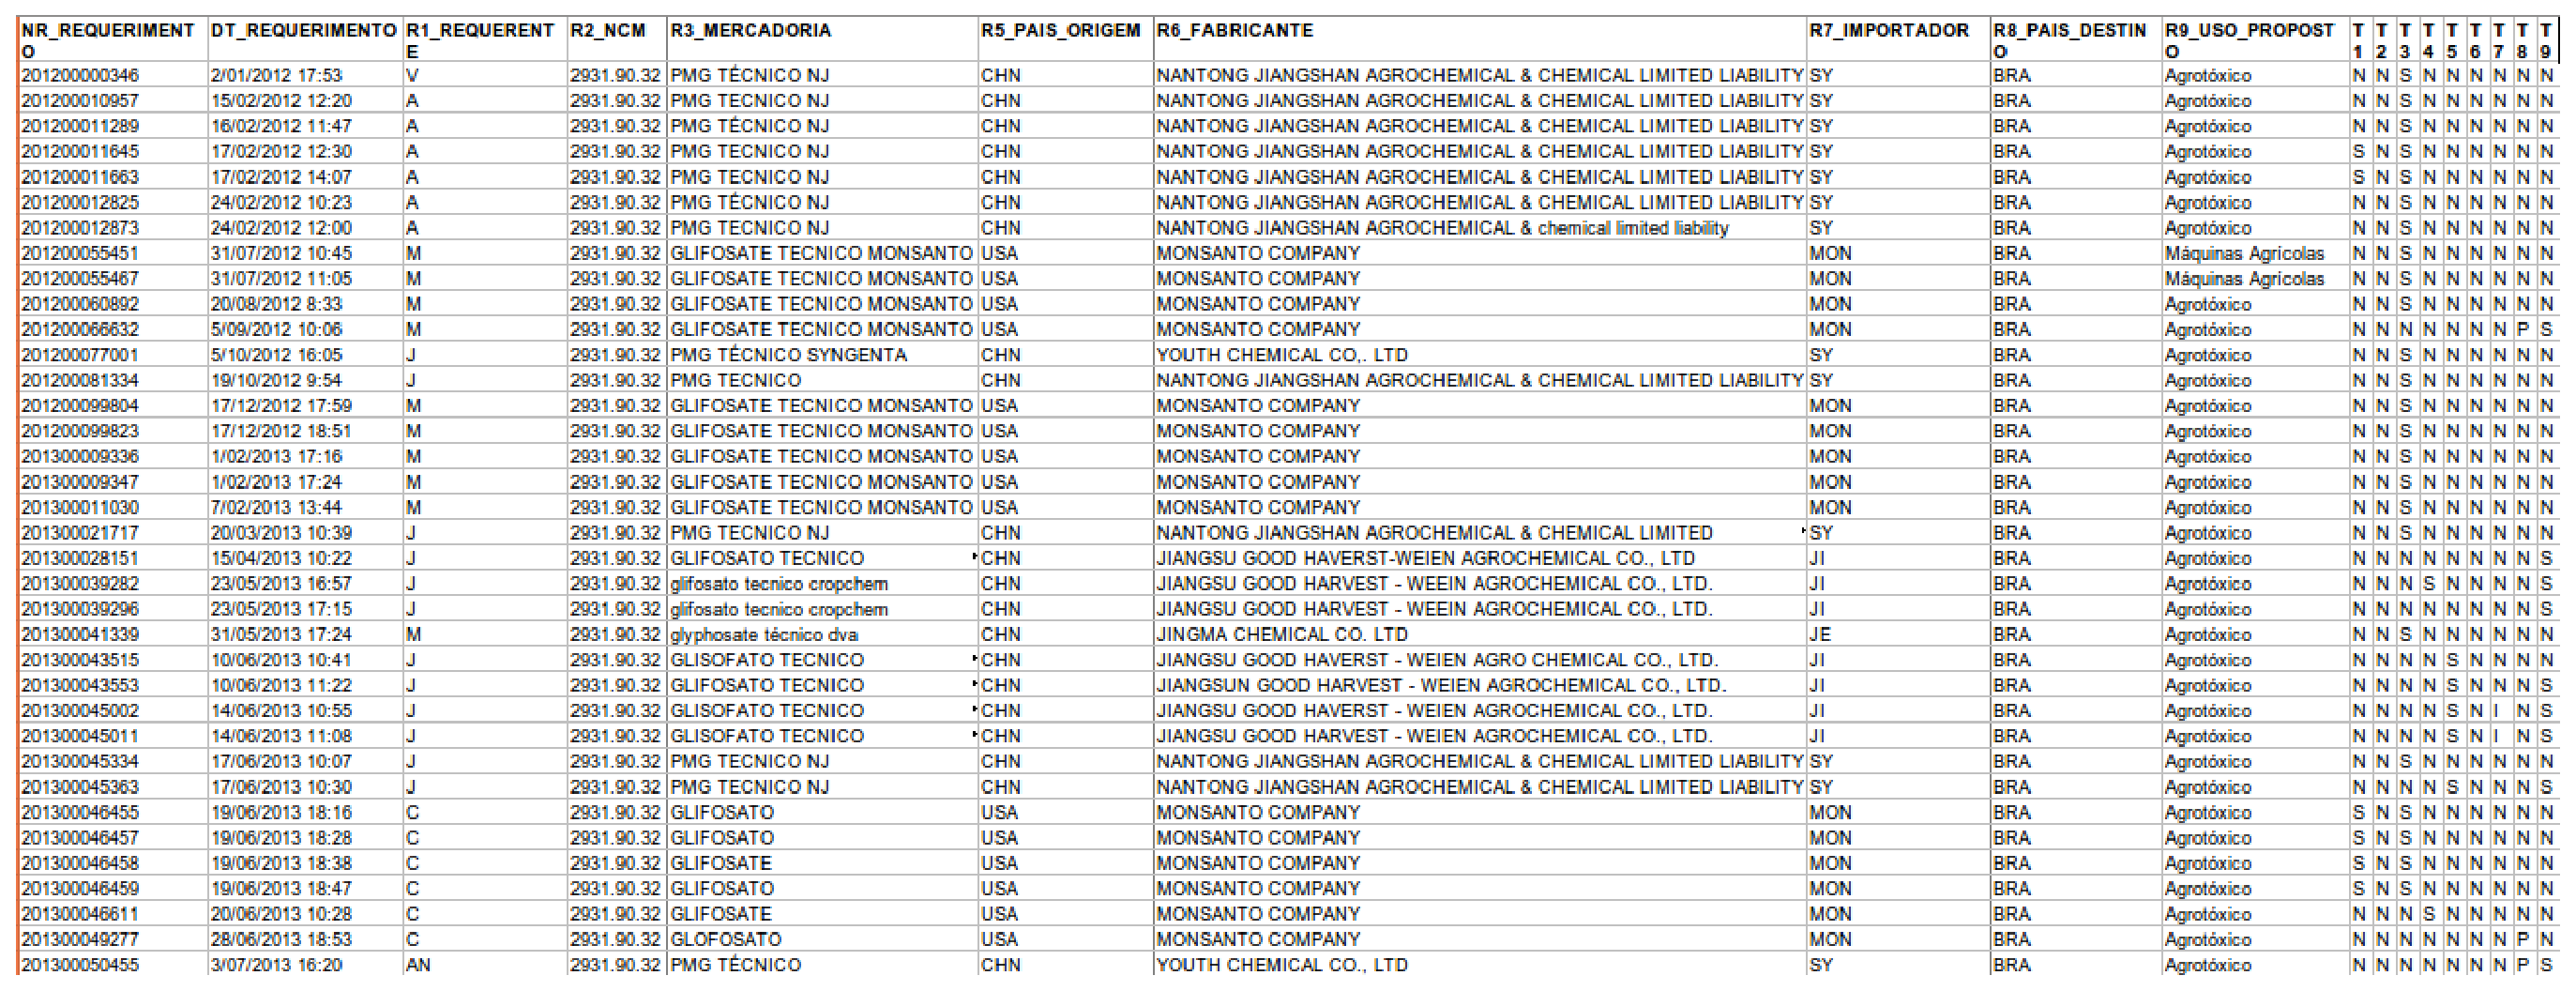
\includegraphics[keepaspectratio=true,scale=0.30]
{figuras/tabelaMapa.eps}
\caption{Dados de Exemplo}
\label{tabelaMapa}
\end{figure}

% Please add the following required packages to your document preamble:
% \usepackage{graphicx}
\begin{table}[h]
\resizebox{\textwidth}{!}{%
\begin{tabular}{|l|l|l|l|}
\hline
Nome            & Tipo                     & Conteúdo               & Descrição                                                                                  \\ \hline
NR REQUERIMENTO & Átomo Numérico           & {[}0 - 999999999999{]} & Identifica unicamente o requerimento. Os quatro primeiro dígitos são o ano do requerimento \\ \hline
DT REQUERIMENTO & Sequência de Categóricos & Texto                  & Momento no tempo em que este requerimento foi feito                                        \\ \hline
R1 REQUERENTE   & Sequência de Categóricos & Texto                  & Identifica unicamente o empresário requerente                                              \\ \hline
R2 NCM          & Sequência de Categóricos & Texto                  & Nomenclatura Comum do Mercosul. Identifica o produto ou categorias de produtos             \\ \hline
R3 MERCADORIA   & Sequência de Categóricos & Texto                  & Nome do produto comercializado                                                             \\ \hline
R5 PAIS ORIGEM  & Átomo Categórico         & Um dos 191 Países      & Sigla que corresponde ao país de origem do produto importado                               \\ \hline
R6 FABRICANTE   & Sequência de Categóricos & Texto                  & Corresponde ao nome da empresa fabricante do produto importado                             \\ \hline
R7 IMPORTADOR   & Sequência de Categóricos & Texto                  & Corresponde ao exportador do produto no país de origem                                     \\ \hline
R9 USO PROPOSTO & Sequência de Categóricos & Texto                  & Objetivo de utilização do produto importado                                                \\ \hline
T1              & Átomo Categórico         & {[}N ou S{]}           & Falta de autorização                                                                       \\ \hline
T2              & Átomo Categórico         & {[}N ou S{]}           & Problema no Certificado Zoosanitário, Sanitário ou Fitosanitário                           \\ \hline
T3              & Átomo Categórico         & {[}N ou S{]}           & Outras inconformidades documentais                                                         \\ \hline
T4              & Átomo Categórico         & {[}N ou S{]}           & Problema na embalagem do produto                                                           \\ \hline
T5              & Átomo Categórico         & {[}N ou S{]}           & Problema na higiene, armazenamento ou transporte
\\ \hline
T6              & Átomo Categórico         & {[}N ou S{]}           & Problema no rótulo ou na etiqueta do produto                                               \\ \hline
T7              & Átomo Categórico         & {[}N ou S{]}           & Problema na identidade ou quantidade do produto                                            \\ \hline
T8              & Átomo Categórico         & {[}N ou S{]}           & Problema de doença, infestação ou praga                                                    \\ \hline
T9              & Átomo Categórico         & {[}N ou S{]}           & Problema com outras inconformidades físicas                                                \\ \hline
\end{tabular}
}
\caption{Descrição dos Dados do MAPA}
\label{my-label}
\end{table}

Os dois primeiros atributos, "NR REQUERIMENTO" e "DT REQUERIMENTO" dizem respeito a informações que são da instância do dado em si. Estas informações são geradas na hora do registro dos dados e não possuem relação direta com o contexto do problema.

Todos os atributos que começam com a letra "R" são relativos a informações do Requerimento. Estas informações identificam a requisição de importação, mostrando características do produto, do fabricante, do requerente e do importador.

Os atributos que começam com a letra "T" são referentes aos Termos de Ocorrência dos requerimentos. Os atributos "T1", "T2" e "T3" são correspondentes a inconformidades documentais que podem acontecer no processo do requerimento. Os outros atributos do tipo "T" representam inconformidades físicas que se mostram nos produtos.

Este conjunto de dados está em formato bruto e é suscetível a Engenharia de Características. Alguns atributos podem ser transformados para extração de informações e outros podem ser omitidos, pois não possuem relacionamento direto com o contexto do problema. 

























